\documentclass[12pt]{article}
            \usepackage{sbc-template}
            \makeatletter
            \renewcommand{\inst}[1]{}
            \makeatother
            \usepackage{graphicx,url}
            \usepackage[utf8]{inputenc}
            \usepackage[T1]{fontenc}
            \usepackage[brazil]{babel}
            \usepackage{longtable,booktabs,array,tabularx}
            \usepackage{amsmath,amssymb}
            \usepackage{fvextra}
            \newcolumntype{Y}{>{\raggedright\arraybackslash}X}
            \newcolumntype{C}{>{\centering\arraybackslash}X}
            \setlength{\LTleft}{0pt}
            \setlength{\LTright}{0pt}
            \RecustomVerbatimEnvironment{verbatim}{Verbatim}{%
              breaklines=true,
              breakanywhere=true,
              breaksymbolleft={},
              fontsize=\small
            }
            \providecommand{\tightlist}{%%
              \setlength{\itemsep}{0pt}\setlength{\parskip}{0pt}}
            \providecommand{\pandocbounded}[1]{#1}
            \usepackage{fancyhdr}
            \pagestyle{fancy}
            \fancyhf{}
            \fancyfoot[R]{\thepage}
            \fancyfoot[L]{SANTOS, Anderson F. P. dos — Avaliação e boas práticas}
            \renewcommand{\headrulewidth}{0pt}
            \renewcommand{\footrulewidth}{0.4pt}
            \sloppy
            \title{Avaliação e boas práticas}
            \author{Anderson Fernandes Pereira dos Santos}
            \address{Instituto Militar de Engenharia (IME), Rio de Janeiro, Brazil \\
Venturus Innovation Center, Campinas, Brazil \\
\texttt{anderson@ime.eb.br} | \texttt{anderson.santos@venturus.org.br}}
            \begin{document}

            \maketitle

            \begin{resumo}
            Este artigo organiza o benchmark central da série. O objetivo não é apenas mostrar uma tabela final, mas ensinar como comparar modelos de séries temporais de forma justa quando o interesse e chegar até RC e QRC sem perder contato com técnicas clássicas fortes. Por isso, o texto formaliza o protocolo experimental, resume as implementações já construídas no projeto, apresenta as equações mínimas das famílias avaliadas e discute o benchmark consolidado real no recorte adotado no Favorita. O resultado mais importante e metodológico: \texttt{ETS}, \texttt{XGBoost} e \texttt{Prophet} formam uma referencia forte que impede avaliar RC e QRC contra baselines fracos.
            \end{resumo}

            \section{O que o leitor vai aprender}\label{1-o-que-o-leitor-vai-aprender}

Ao final deste artigo, você será capaz de:

\begin{enumerate}
\def\labelenumi{\arabic{enumi}.}
\tightlist
\item
  comparar modelos temporais com um protocolo realmente comum;
\item
  entender o papel de cada família de modelo no benchmark;
\item
  ler uma tabela comparativa sem cair em conclusoes apressadas;
\item
  reproduzir o benchmark com os scripts do projeto;
\item
  usar os resultados clássicos como referencia seria para RC e QRC.
\end{enumerate}

\section{Por que avaliação em séries temporais e delicada}\label{2-por-que-avaliauxe7uxe3o-em-suxe9ries-temporais-e-delicada}

Em séries temporais, avaliação injusta aparece facilmente:

\begin{itemize}
\tightlist
\item
  quando um modelo usa um split temporal diferente;
\item
  quando features usam informação do futuro;
\item
  quando um modelo recebe regressoras exógenas e outro não;
\item
  quando os horizontes de previsão não coincidem;
\item
  quando as métricas destacadas mudam de um experimento para outro.
\end{itemize}

Para evitar isso, este projeto fixa o seguinte principio:

\[
\text{mesmo recorte} + \text{mesmo split} + \text{mesmas métricas} = \text{comparação honesta}.
\]

\section{Protocolo experimental da série}\label{3-protocolo-experimental-da-suxe9rie}

\subsection{Recorte comum}\label{31-recorte-comum}

Todos os modelos usam:

\begin{itemize}
\tightlist
\item
  \texttt{store\_nbr\ =\ 1}
\item
  \texttt{family\ =\ BEVERAGES}
\item
  frequência diária
\item
  últimos \texttt{90} dias como teste
\end{itemize}

\subsection{Regra de split}\label{32-regra-de-split}

Formalmente:

\[
\mathcal{D}_{train} = \{(x_t, y_t)\}_{t=1}^{T-90},
\qquad
\mathcal{D}_{test} = \{(x_t, y_t)\}_{t=T-89}^T.
\]

\subsection{Modelos avaliados}\label{33-modelos-avaliados}

\begin{verbatim}
\begin{table}[htbp]
\centering
\small
\begin{tabularx}{\linewidth}{@{}lYY@{}}
\toprule
Modelo & Implementacao & Ideia central \\
\midrule
Seasonal Naive & \path{code/baselines/seasonal_naives/} & repete a ultima semana observada \\
ETS & \path{code/baselines/ets/} & modelo de nivel, tendencia e sazonalidade aditiva \\
Prophet & \path{code/baselines/prophet/} & decomposicao de tendencia, sazonalidade e regressor exogeno \\
XGBoost & \path{code/classical/xgboost/} & aprendizado tabular sobre lags e medias moveis \\
LSTM & \path{code/classical/lstm/} & rede recorrente treinada por gradiente \\
RC & \path{code/rc/} & reservatorio fixo e readout linear \\
QRC & \path{code/qrc/} & reservatorio quantico implementado com Qiskit \\
\bottomrule
\end{tabularx}
\end{table}
\end{verbatim}

\subsection{Métricas avaliadas}\label{34-muxe9tricas-avaliadas}

O benchmark usa:

\[
\mathrm{MAE},\ \mathrm{RMSE},\ \mathrm{WAPE},\ \mathrm{sMAPE}.
\]

As implementações dessas métricas estao em \texttt{code/common/metrics.py}.

\section{As famílias de modelo em uma pagina}\label{4-as-famuxedlias-de-modelo-em-uma-pagina}

Para manter a comparação didática, vale resumir a lógica de cada família.

\subsection{Seasonal Naive}\label{41-seasonal-naive}

\[
\hat{y}_t = y_{t-7}.
\]

Serve como baseline sazonal mínimo.

\subsection{ETS}\label{42-ets}

O ETS aditivo pode ser resumido por

\[
\ell_t = \alpha (y_t - s_{t-m}) + (1 - \alpha)(\ell_{t-1} + b_{t-1}),
\]
\[
b_t = \beta (\ell_t - \ell_{t-1}) + (1 - \beta) b_{t-1},
\]
\[
s_t = \gamma (y_t - \ell_t) + (1 - \gamma) s_{t-m}.
\]

\subsection{Prophet}\label{43-prophet}

O Prophet modela a série como

\[
y(t) = g(t) + s(t) + h(t) + \beta x_t + \epsilon_t,
\]

em que \texttt{onpromotion} entra como regressor exógeno no projeto.

\subsection{XGBoost}\label{44-xgboost}

O modelo tabular usa lags, médias móveis e calendário para aprender

\[
\hat{y}_t = \sum_{m=1}^M f_m(z_t),
\]

com \(z_t\) contendo \texttt{lag\_1}, \texttt{lag\_7}, \texttt{lag\_14}, \texttt{lag\_28}, médias móveis e calendarios.

\subsection{LSTM}\label{45-lstm}

A LSTM usa portas para atualizar memória:

\[
i_t = \sigma(W_i [h_{t-1}, x_t] + b_i), \quad
f_t = \sigma(W_f [h_{t-1}, x_t] + b_f),
\]
\[
c_t = f_t \odot c_{t-1} + i_t \odot \tilde{c}_t.
\]

\subsection{RC}\label{46-rc}

\[
x_t = (1 - \alpha) x_{t-1} + \alpha \tanh(W_{res} x_{t-1} + W_{in} u_t + b).
\]

\subsection{QRC}\label{47-qrc}

O QRC será detalhado nos artigos 6 e 7, mas aqui ele entra como

\[
z_t^{(j)} = \langle \psi_t | O_j | \psi_t \rangle,
\qquad
\hat{y}_t = W_{out} [1; u_t; z_t].
\]

\section{Benchmark comparativo atual}\label{5-benchmark-comparativo-atual}

A tabela abaixo resume os resultados reais obtidos no projeto.

\begin{longtable}[]{@{}llllll@{}}
\toprule\noalign{}
Modelo & Família & MAE & RMSE & WAPE & sMAPE \\
\midrule\noalign{}
\endhead
\bottomrule\noalign{}
\endlastfoot
ETS & baseline estatístico & 216.303 & 307.638 & 0.0999 & 0.1042 \\
XGBoost & ML clássico & 256.666 & 332.828 & 0.1185 & 0.1237 \\
Prophet & baseline estatístico & 257.584 & 321.818 & 0.1189 & 0.1319 \\
Seasonal Naive & baseline estatístico & 259.067 & 352.280 & 0.1196 & 0.1361 \\
RC & reservoir computing clássico & 324.294 & 423.417 & 0.1498 & 0.1653 \\
LSTM & DL clássico & 371.827 & 461.342 & 0.1717 & 0.1822 \\
QRC14x7 & reservoir computing quântico & 441.286 & 525.325 & 0.2038 & 0.2269 \\
QRC8x5 & reservoir computing quântico & 455.833 & 526.949 & 0.2105 & 0.2342 \\
\end{longtable}

Uma leitura ordenada por rank médio reforca a comparação.

\begin{longtable}[]{@{}llllll@{}}
\toprule\noalign{}
Modelo & Rank médio & MAE & RMSE & WAPE & sMAPE \\
\midrule\noalign{}
\endhead
\bottomrule\noalign{}
\endlastfoot
ETS & 1.00 & 216.303 & 307.638 & 0.0999 & 0.1042 \\
XGBoost & 2.25 & 256.666 & 332.828 & 0.1185 & 0.1237 \\
Prophet & 2.75 & 257.584 & 321.818 & 0.1189 & 0.1319 \\
Seasonal Naive & 4.00 & 259.067 & 352.280 & 0.1196 & 0.1361 \\
RC & 5.00 & 324.294 & 423.417 & 0.1498 & 0.1653 \\
LSTM & 6.00 & 371.827 & 461.342 & 0.1717 & 0.1822 \\
QRC14x7 & 7.00 & 441.286 & 525.325 & 0.2038 & 0.2269 \\
QRC8x5 & 8.00 & 455.833 & 526.949 & 0.2105 & 0.2342 \\
\end{longtable}

\begin{figure}[htbp]
\centering
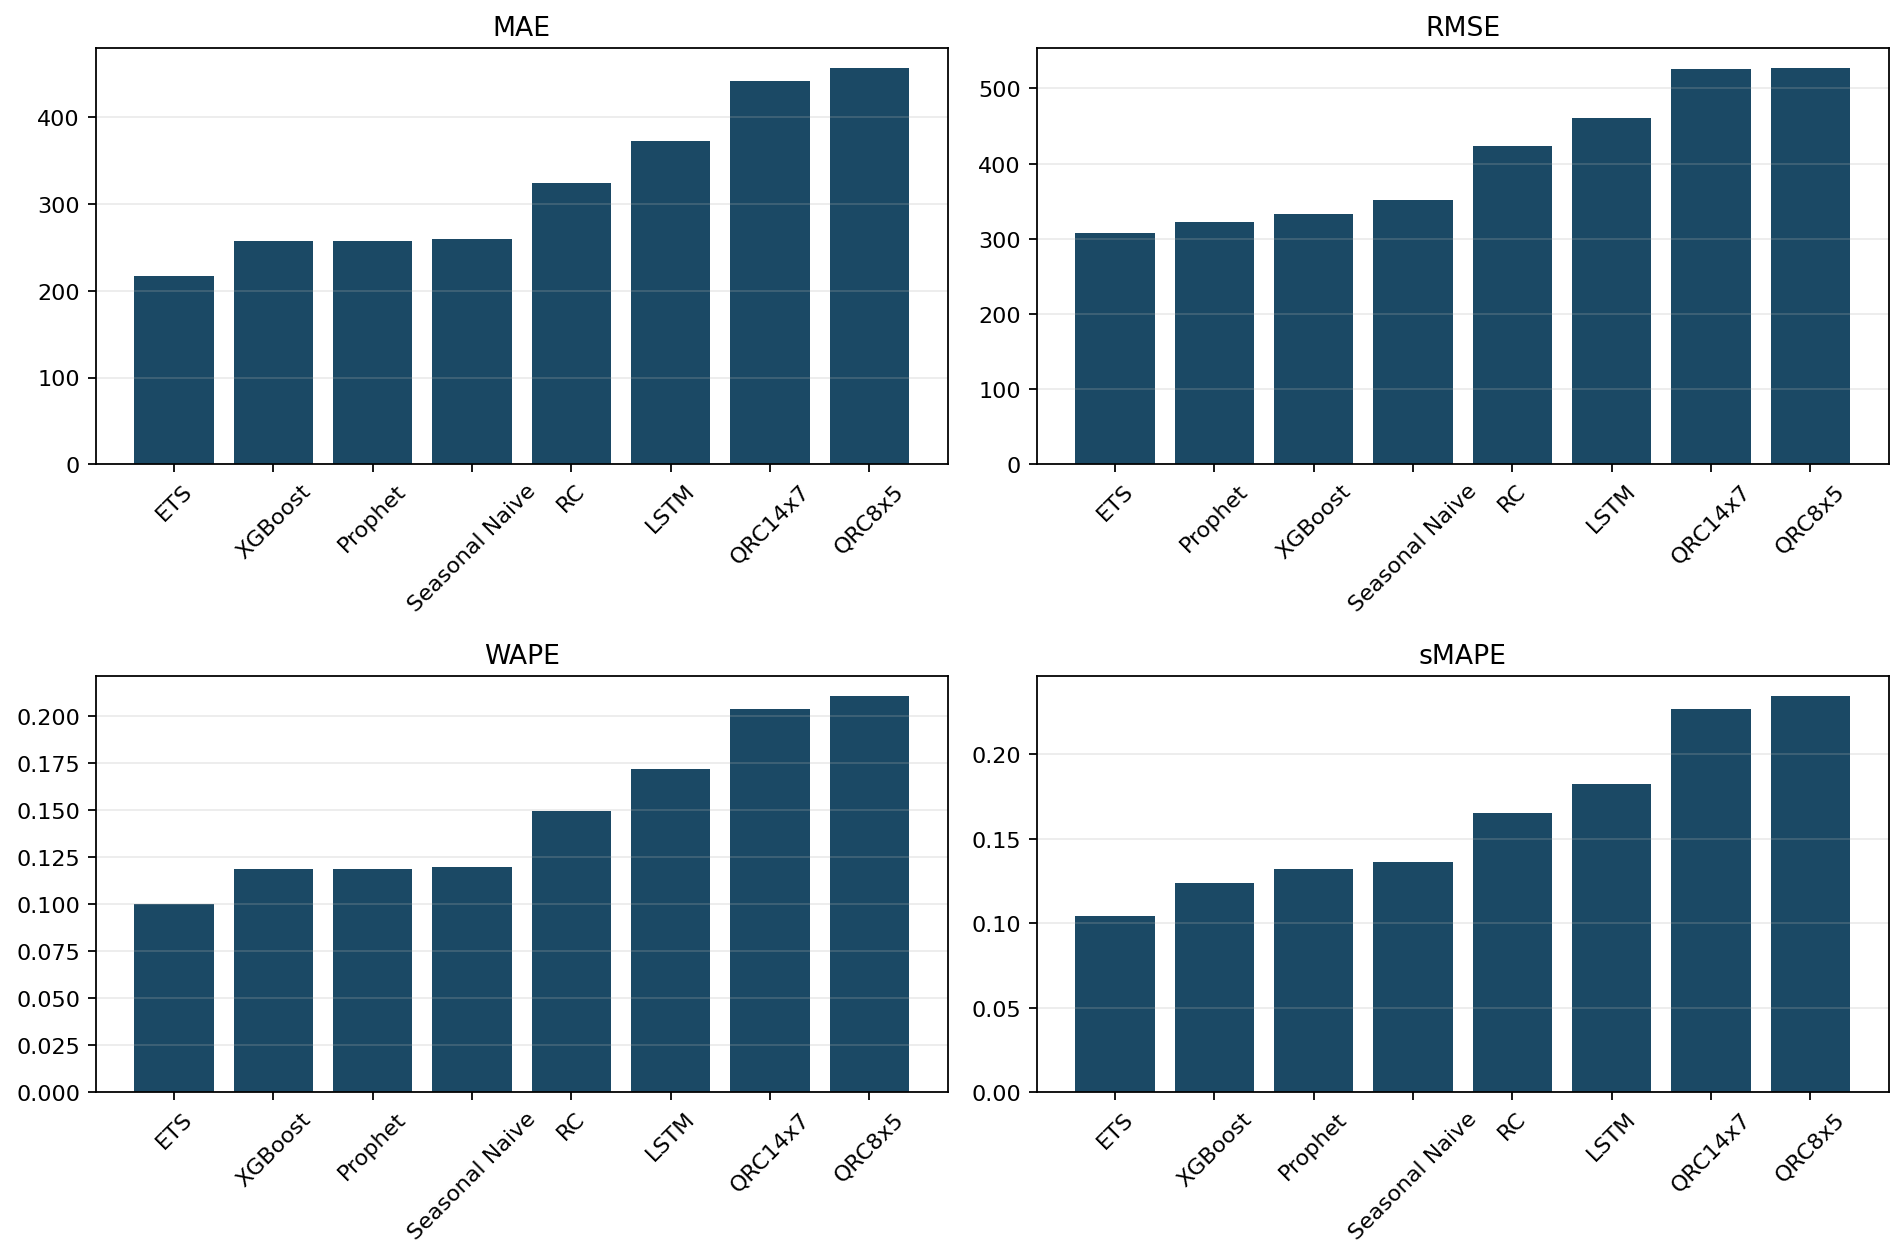
\includegraphics[width=\linewidth,keepaspectratio]{computational_results_20260402_222902/benchmark_metric_bars.png}
\caption{Comparação visual das métricas do benchmark completo.}
\end{figure}

\begin{figure}[htbp]
\centering
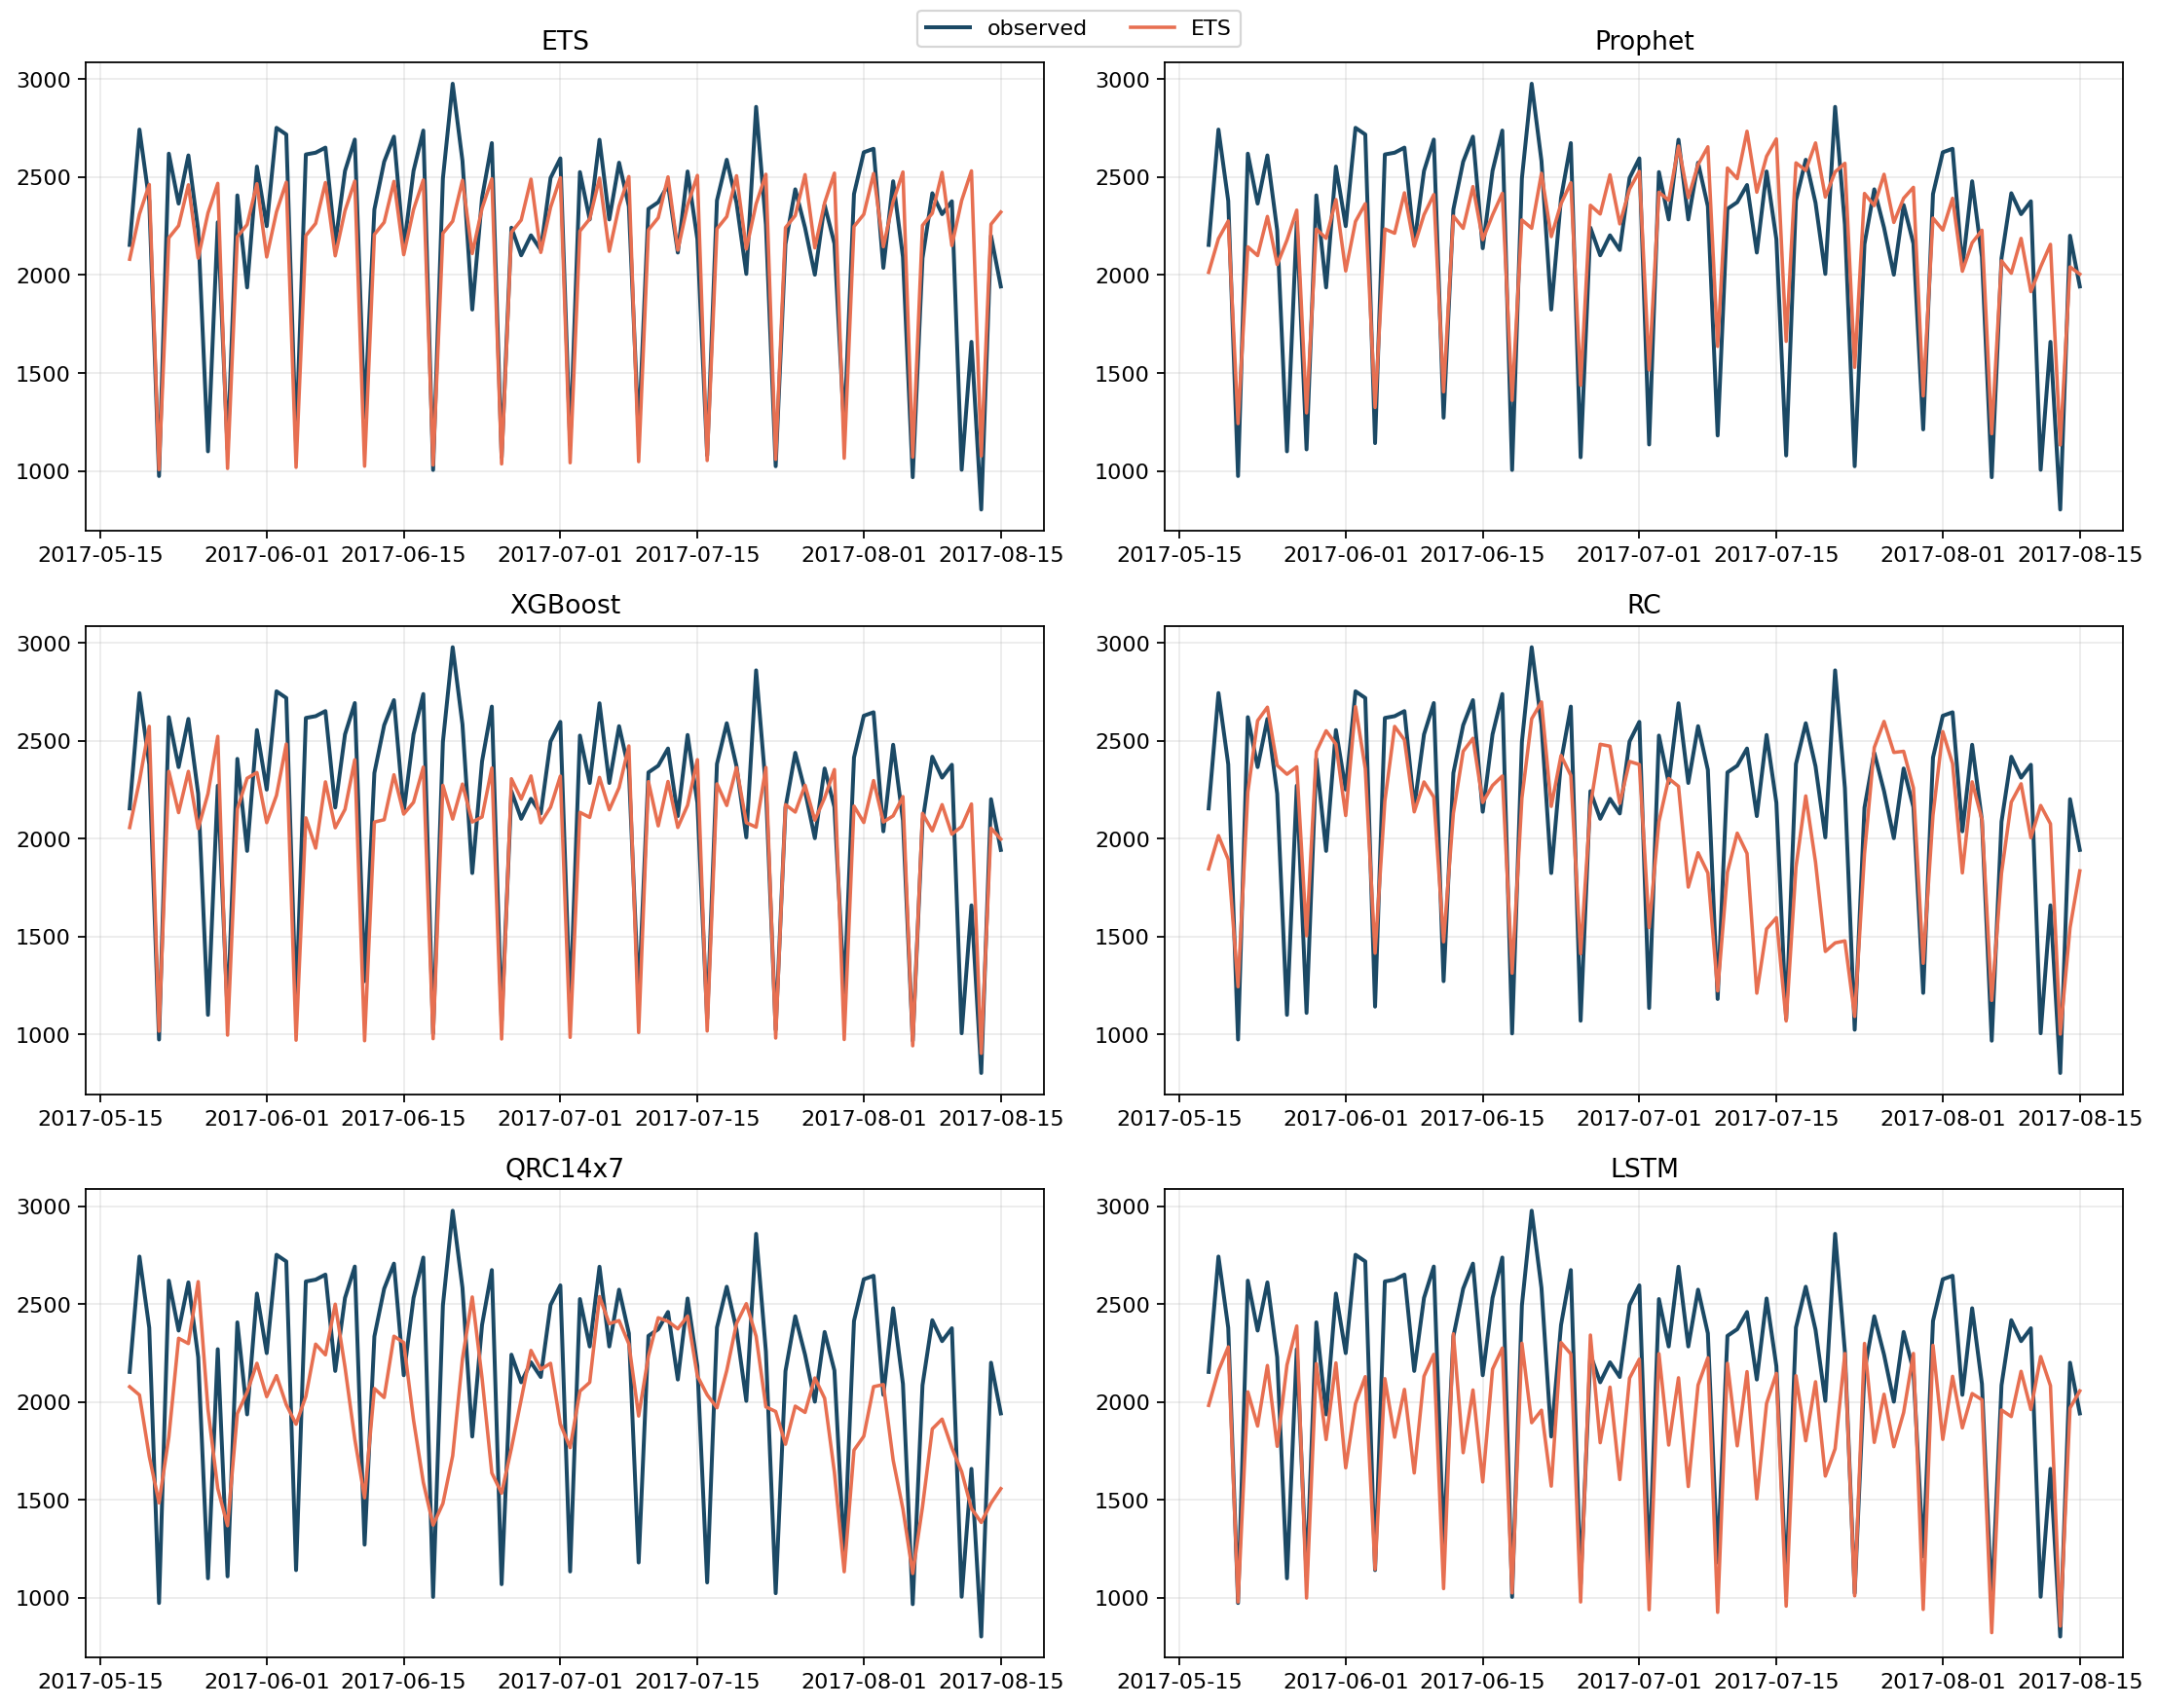
\includegraphics[width=\linewidth,keepaspectratio]{computational_results_20260402_222902/benchmark_forecast_grid.png}
\caption{Grade de previsões dos diferentes modelos no mesmo bloco de teste.}
\end{figure}

\section{Leitura dos resultados}\label{6-leitura-dos-resultados}

\subsection{ETS na lideranca}\label{61-ets-na-lideranca}

O \texttt{ETS} foi o melhor modelo no recorte em todas as métricas principais. Isso é importante porque mostra que um baseline estatístico bem implementado continua sendo uma referencia difícil de bater.

\subsection{XGBoost e Prophet como faixa intermediária forte}\label{62-xgboost-e-prophet-como-faixa-intermediuxe1ria-forte}

\texttt{XGBoost} e \texttt{Prophet} formam uma segunda faixa de desempenho. Ambos ficaram muito próximos do \texttt{Seasonal\ Naive} em algumas métricas, mas entregaram um pacote mais robusto no conjunto do benchmark.

\subsection{O que o RC entrega}\label{63-o-que-o-rc-entrega}

O \texttt{RC} superou a \texttt{LSTM}, o que é pedagogicamente interessante. Em um setup pequeno e pouco ajustado, uma rede recorrente treinada por gradiente não vence automaticamente um reservatório fixo.

\subsection{O que o QRC entrega}\label{64-o-que-o-qrc-entrega}

O \texttt{QRC} funcionou de ponta a ponta e foi comparado no mesmo recorte de dados. No entanto, ficou abaixo das técnicas clássicas neste benchmark. Isso não invalida o estudo; ao contrario, torna a comparação mais honesta.

\section{O que significa uma comparação justa}\label{7-o-que-significa-uma-comparauxe7uxe3o-justa}

Este benchmark só é didaticamente útil porque respeita três regras:

\begin{enumerate}
\def\labelenumi{\arabic{enumi}.}
\tightlist
\item
  todos os modelos usam os mesmos dados;
\item
  todos produzem previsão para os mesmos \texttt{90} dias;
\item
  todos sao julgados pelas mesmas métricas.
\end{enumerate}

Isso evita a narrativa enganosa de que um modelo "venceu" porque recebeu mais contexto ou uma tarefa mais fácil.

\section{Passo-a-passo para reproduzir o benchmark}\label{8-passo-a-passo-para-reproduzir-o-benchmark}

A reprodução pode ser feita em lotes, executando um script por família:

\begin{verbatim}
python code/baselines/seasonal_naives/run.py
python code/baselines/ets/run.py
python code/baselines/prophet/run.py
python code/classical/xgboost/run.py
python code/classical/lstm/run.py
python code/rc/run.py
python code/qrc/run.py
\end{verbatim}

Os testes associados seguem a mesma organização:

\begin{verbatim}
pytest code/baselines/seasonal_naives/test_model.py
pytest code/baselines/ets/test_model.py
pytest code/baselines/prophet/test_model.py
pytest code/classical/xgboost/test_model.py
pytest code/classical/lstm/test_model.py
pytest code/rc/test_model.py
pytest code/qrc/test_model.py
pytest code/qrc/test_objective.py
\end{verbatim}

\section{Checklist de boas praticas}\label{9-checklist-de-boas-praticas}

O artigo deixa um checklist mínimo para os próximos experimentos:

\begin{itemize}
\tightlist
\item
  manter o split temporal fixo;
\item
  registrar métricas em arquivo;
\item
  salvar previsões e figuras;
\item
  documentar hiperparâmetros;
\item
  não comparar RC e QRC apenas com baselines fracos.
\end{itemize}

\section{Regras herdadas para a fase QRC}\label{10-regras-herdadas-para-a-fase-qrc}

Quando chegarmos ao QRC, duas regras deste benchmark continuam valendo:

\begin{enumerate}
\def\labelenumi{\arabic{enumi}.}
\tightlist
\item
  o QRC deve ser comparado com as técnicas clássicas já implementadas;
\item
  o mesmo recorte de dados deve ser mantido, mesmo que o reservatório quântico simplifique sua representação interna.
\end{enumerate}

Isso é o que transforma o estudo final em um artigo de ensino serio, e não em uma demonstracao isolada.

\section{Conclusão}\label{11-conclusuxe3o}

O benchmark consolidado da série esta agora estabelecido. Ele mostra que a competição relevante para RC e QRC não é contra referencias artificiais, mas contra modelos clássicos fortes e bem executados. Isso torna a rota até QRC intelectualmente mais exigente, mas também muito mais valiosa.

\section*{Entregaveis associados no repositorio}\label{entregaveis-associados-no-repositorio}

\begin{itemize}
\tightlist
\item
  benchmark consolidado: \texttt{code/RESULTS.md}
\item
  implementações de baseline: \texttt{code/baselines/}
\item
  implementações clássicas: \texttt{code/classical/}
\item
  implementação de RC: \texttt{code/rc/}
\item
  implementação de QRC: \texttt{code/qrc/}
\item
  artefatos comparativos deste artigo: \texttt{computational\_results\_20260402\_222902/}
\end{itemize}

\section{Referências}\label{referencias}

\begin{thebibliography}{9}

\bibitem{jaeger2001}
JAEGER, H. \textbf{The ``echo state'' approach to analysing and training recurrent neural networks}. Bonn: German National Research Center for Information Technology (GMD), 2001.

\bibitem{lukosevicius2009}
LUKOSEVICIUS, M.; JAEGER, H. \textbf{Reservoir computing approaches to recurrent neural network training}. \emph{Computer Science Review}, v. 3, n. 3, p. 127--149, 2009.

\bibitem{lukosevicius2012}
LUKOSEVICIUS, M. \textbf{A practical guide to applying echo state networks}. In: MONTAVON, G.; ORR, G. B.; MÜLLER, K.-R. (org.). \emph{Neural Networks: Tricks of the Trade}. 2. ed. Berlin: Springer, 2012. p. 659--686.

\bibitem{fujii2017}
FUJII, K.; NAKAJIMA, K. \textbf{Harnessing disordered-ensemble quantum dynamics for machine learning}. \emph{Physical Review Applied}, v. 8, n. 2, 024030, 2017.

\end{thebibliography}

            \end{document}
